\chapter{Lineární regrese}

\section{Příklady lineární regrese}

\begin{example}
Vzdálenost $s$, kterou částice urazí v čase $t$ je dána rovnicí $s = \beta_0 + \beta_1t$, kde $\beta_1$ je průměrnou rychlostí a $\beta_0$ je pozice v čase $t = 0$. Jestliže $\beta_0$ a $\beta_1$ neznáme, pak lze pozorovat $s$ pro dvě rozdílná $t$ a z odpovídajících dvou rovnic vyřešit $\beta_0$ a $\beta_1$. Pokud např. $s = 2$ pro $t = 1$ a $s = 11$ pro $t = 4$, získáme rovnice $2 = \beta_0 + \beta_1$ a $11 = \beta_0 + 4 \beta_1$, jejichž řešením je $\beta_0 = -1$ a $\beta_1 = 3$, tj. $s = -1 + 3t$.

Předpokládejme, že měření vzdálenosti je zatíženou náhodnou chybou. Proto namísto $s$ pozorujeme $Y = s + E$, kde $E$ představuje chybu s nulovou střední hodnotou. Substitucí za $s$ tak získáme
\begin{equation*}
Y = \beta_0 + \beta_1t + E
\end{equation*}
kde $Y$ je náhodná veličina, jejíž realizaci jsme schopni pozorovat, a $E$ je náhodná veličina, jejíž realizaci schopni pozorovat nejsme. $t$ je nenáhodná veličina a $\beta_0$ a $\beta_1$ představují neznámé parametry. Hodnotu $\beta_0$ a $\beta_1$ nejsme schopni vypočíst ze dvou pozorování $(t,Y)$, jako tomu bylo v případě $(t, s)$, protože neexistuje žádná funkční závislost mezi $Y$ a $t$. Cílem našeho snažení je nalézt $\beta_0$ a $\beta_1$ a odvodit tak vztah $s = \beta_0 + \beta_1t$ pro různé hodnoty $t$. Protože $s$ je zatíženo chybami a nelze ho přímo pozorovat, nemůžeme znát ani $\beta_0$ a $\beta_1$. Nicméně na základě pozorování různých $(t,Y)$ lze s využitím statistických metod odhadnout $\beta_0$, $\beta_1$ a $s$.
\end{example}

\begin{example}
Uvažujme vztah mezi výškou jedince $h$ a jeho hmotností $w$. Je zřejmé, že neexistuje žádný funkční vztah mezi $h$ a $w$, nicméně se dá očekávat, že mezi nimi existuje určitá závislost.

Předpokládejme, že výška a váha jsou náhodné veličiny $(W,H)$, které sledují dvourozměrné normální rozdělení. Očekávaná hodnota $H$ pro danou hodnotu $w$ náhodné veličiny $W$, je dána vztahem
\begin{equation*}
E[H|W = w] = \beta_0 + \beta_1 w
\end{equation*}
kde $\beta_0$ a $\beta_1$ jsou parametry dvourozměrného normálního rozdělení. Ačkoliv mezi $H$ a $W$ neexistuje funkční vztah, existuje mezi nimi, pokud předpokládáme sdruženě normální rozdělení, lineární závislost. Proto platí
\begin{equation*}
E[H|W = w] = \beta_0 + \beta_1w
\end{equation*}
nebo také
\begin{equation*}
H_w = \beta_0 + \beta_1 w + E
\end{equation*}
kde $E$ je chyba, která sleduje normální rozdělení.
\end{example}

\section{Definice regresního modelu}

Uvažujme lineární funkci $\mu(\cdot)$ reálné proměnné $x$, tj. $\mu(x) = \beta_0 + \beta_1 x$, kde $x \in D$. Množina $D$ je obykle reprezentována celou reálnou přímkou popř. polopřímkou nebo intervalem. Předpokládejme, že existuje taková rodina kumulativních distribučních funkcí (pro každé $x$ jedna), jejichž střední hodnota pro dané $x = x_0$ je rovna $\beta_0 + \beta_1 x_0$. To znamená, že střední hodnoty těchto kumulativních distribučních funkcí tvoří přímku definovanou jako $\mu(x) = \beta_0 + \beta_1x$, jak je ilustorováno obrázkem (\ref{linear-model}).

\begin{figure}[htp]
\centering
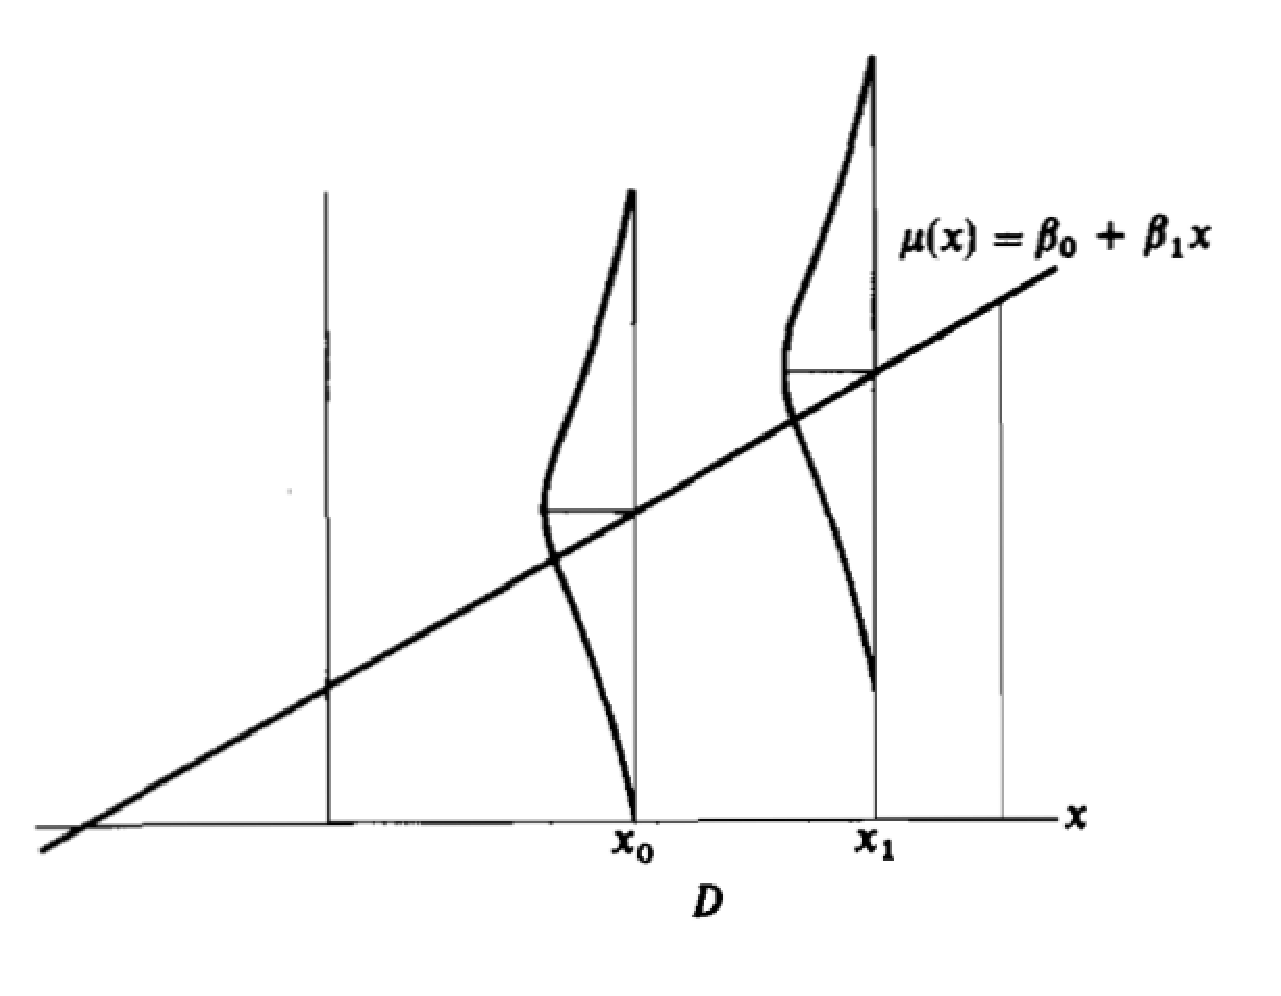
\includegraphics[scale = 0.5]{pictures/linear_model.eps}
\caption{Lineární regrese}
\label{linear-model}
\end{figure}

Cílem je na základě náhodného výběru z několika těchto kumulativních distribučních funkcí získat odhad parametrů $\beta_0$ a $\beta_1$. Toho je dosaženo následovně.
\begin{enumerate}
\item Soubor $n$ pozorování hodnot $x$ označme jako $x_1, ..., x_n$. Soubor $x_1, ..., x_n$ není souborem náhodných veličin, nicméně může být vybrán jak náhodně tak na základě vědomé selekce.
\item Každé $x_i$ určuje kumulativní distribuční funkci se střední hodnotou $\beta_0 + \beta_1 x_i$ a rozptylem $\sigma^2$. Z této kumulativní distribuční funkce je náhodně vybrána jedna hodnota označovaná jako $Y_i$. Tímto způsobem získáme $n$ uspořádaných dvojic $(Y_1, x_1), ... (Y_n, x_n)$. V předchozím textu jsme předpokládali
\begin{equation*}
E[Y_i] = \beta_0 + \beta_1 x_i ~~~ D[Y_i] = \sigma^2
\end{equation*}
Proto jsme schopni definovat náhodné veličiny $E_1, ..., E_n$ jako
\begin{equation*}
E_i = Y_i - \beta_0 - \beta_1 x_i, ~~~ i = 1, ..., n
\end{equation*}
kde $E[E_i] = 0$ a $D[E] = \sigma^2$.
\end{enumerate}
Výše uvedený vztah lze převést do tvaru
\begin{equation*}
Y_i = \beta_0 + \beta_1 x_i + E_i, ~~~ i = 1, ..., n
\end{equation*}
kde $E[E_i] = 0$ a $D[E_i] = \sigma^2$, což je definice jednoduché lineární regrese.

\begin{definition}[Lineární regrese]
Uvažujme funkci $\mu(x) = \beta_0 + \beta_1x$ pro všechna $x \in D$. Pro každé $x$ z $D$ uvažujme kumulativní distribuční funkci $F_{Y_x}(\cdot)$ se střední hodnotou $\mu(x) = \beta_0 + \beta_1 x$ a rozptylem $\sigma^2$. Nechť $x_1, ..., x_n$ představuje soubor $n$ (nikoliv nutně náhodných) pozorování z $D$. Pro $x_i$ uvažujme jednoprvkový náhodný výběr $Y_i$ z $F_{Y_{x_i}}(\cdot)$, kde $i = 1, ..., n$. Pak $(Y_1, x_1), ..., (Y_n, x_n)$ představuje soubor $n$ uspořádaných dvojic, které jsou ``provázány'' vztahem
\begin{equation*}
E[Y_i] = \beta_0 + \beta_1 x_i
\end{equation*}
a
\begin{equation*}
D[Y_i] = \sigma^2
\end{equation*}
kde $i = 1, ..., n$. Výše uvedené rovnice je možné vyjádřit také ve tvaru
\begin{gather*}
Y_i = \beta_0 + \beta_1 x_i + E_i\\
E[E_i] = 0\\
D[E_i] = \sigma^2
\end{gather*}
kde $i = 1, ..., n$.

Tyto vztahy a podmínky definují jednoduchý regresní model.
\end{definition}

Slovo ``lineární'' v pojmu ``lineární regrese'' odpovídá skutečnosti, že funkce $\mu(\cdot)$ je lineární v parametrech $\beta_0$ a $\beta_1$. Proto je $Y = \mu(x) + E$, kde $\mu(x) = \beta_0 + \beta_1 e^x$, také lineární regresí. Na kumulativní distribuční funkci $F_{Y_x}(\cdot)$ jsou zpravidla kladeny další požadavky jako např. normalita. Dále je způsob náhodného výběru takový, že $Y_i$ jsou buďto sdruženě nezávislé nebo párově nezávislé. Tímto se dostáváme k definici dvou základních případů, na které se budeme odkazovat v následujících kapitolách.

\begin{itemize}
\item \textbf{Případ A} - V tomto případě je všech $n$ náhodných veličin $Y_i$ sdruženě nezávislých a každé $Y_i$ sleduje normální rozdělení.
\item \textbf{Případ B} - V tomto případě jsou $Y_i$ párově nezávislé, tj. $cov(Y_i, Y_j) = 0$ pro všechna $i \neq j = 1, ..., n$.
\end{itemize}

Pro případ A budeme diskutovat
\begin{enumerate}
\item bodový odhad $\beta_0, \beta_1, \sigma^2$ a $\mu(x)$ pro libovolné $x \in D$
\item interval spolehlivosti pro $\beta_0, \beta_1, \sigma^2$ a $\mu(x)$ pro libovolné $x \in D$
\item testování hypotéz pro $\beta_0, \beta_1$ a $\sigma^2$
\end{enumerate}

Pro případ B budeme diskutovat
\begin{enumerate}
\item bodový odhad $\beta_0, \beta_1, \sigma^2$ a $\mu(x)$ pro libovolné $x \in D$
\end{enumerate}

\section{Bodový odhad - případ A}

V tomto případě jsou $Y_1, ..., Y_n$ nezávislé normální veličiny se středními hodnotami $\beta_0 + \beta_1 x_1, ..., \beta_0 + \beta_1 x_n$ a rozptylem $\sigma^2$. Pro účely bodového odhadu použijeme metodu maximální věrohodnosti. Věrohodnostní funkce má tvar
\begin{equation}
L(\beta_0, \beta_1, \sigma^2) = L(\beta_0, \beta_1, \sigma^2; y_1, ..., y_n)\\
= \prod_{i = 1}^n\left(\frac{1}{\sqrt{2 \pi} \sigma}e^{-\frac{1}{2}\left(\frac{y_i - \beta_0 - \beta_1x_i}{\sigma}\right)^2}\right)
\end{equation}
a
\begin{equation*}
\ln\left(L(\beta_0, \beta_1, \sigma^2)\right) = - \frac{n}{2}\ln(2 \pi) - \frac{n}{2}\ln(\sigma^2) - \frac{1}{2 \sigma^2} \sum_{i = 1}^n(y_i - \beta_0 - \beta_1 x_i)^2
\end{equation*}
V dalším kroku jsou parciální derivace $\ln\left(L(\beta_0, \beta_1, \sigma^2)\right)$ vzhledem k $\beta_0, \beta_1$ a $\sigma^2$ položeny rovno nule. Řešení těchto tří rovnic označme jako $\hat{\beta}_0, \hat{\beta}_1$ a $\tilde{\sigma}^2$. Tyto tři rovnice mají po určitých zjednodušeních tvar
\begin{gather}
\sum_{i = 1}^n (y_i - \hat{\beta}_0 - \hat{\beta}_1 x_i) = 0\\
\sum_{i = 1}^n (y_i - \hat{\beta}_0 - \hat{\beta}_1 x_i)x_i = 0\\
\sum_{i = 1}^n (y_i - \hat{\beta}_0 - \hat{\beta}_1 x_i)^2 = n \tilde{\sigma}^2
\end{gather}
První dvě rovnice jsou lineární v parametrech $\beta_0$ a $\beta_1$, a proto z nich lze tyto parametry relativně jednoduše určit. Dosazením takto vypočtených hodnot do třetí rovnice lze vypočíst $\sigma^2$. Řešení má pak konkrétně podobu
\begin{gather}
\hat{\beta}_1 = \frac{\sum_{i = 1}^n (y_i - \overline{y})(x_i - \overline{x})}{\sum_{i = 1}^n (x_i - \overline{x})^2}\\
\hat{\beta}_0 = \overline{y} - \hat{\beta}_1 \overline{x}\\
\tilde{\sigma}^2 = \frac{1}{n} \sum_{i = 1}^n (y_i - \hat{\beta}_0 - \hat{\beta}_1 x_i)^2
\end{gather}

Protože
\begin{multline*}
f_{Y_i}(y_i; \beta_0, \beta_1, \sigma) = \frac{1}{\sqrt{2 \pi}\sigma} e^{-\frac{1}{2}\left(\frac{y_i - \beta_0 - \beta_1x_i}{\sigma}\right)^2}\\
= \frac{1}{\sqrt{2 \pi} \sigma}e^{-\frac{1}{2 \sigma^2}(\beta_0 + \beta_1x_i)^2}e^{-\frac{1}{2 \sigma^2}y_i^2 + \frac{\beta_0}{\sigma^2}y_i + \frac{\beta_1}{\sigma^2}x_i y_i}
\end{multline*}
je $f_{Y_i}(y_i; \beta_0, \beta_1, \sigma)$ členem tří parametrické exponenciální rodiny pravděpodobnostních rozdělení. Pro na základě zobecněné věty (7.19) přestavují
\begin{equation}
\sum_{i = 1}^n Y_i^2 ~~~ \sum_{i = 1}^n Y_i ~~~ \sum_{i = 1}^n x_i Y_i
\end{equation}
soubor minimálních dostatečných a sdruženě kompletních statistik. Navíc (10.8) je transformací jedna ku jedné statistik (10.2), (10.3) a (10.4), a proto jsou taktéž minimální dostatečné a sdruženě kompletní.

Pokusme se nalézt sdružené pravděpodobnostní rozdělení statistik odpovídajících $\hat{\beta}_0, \hat{\beta}_1$ a $\tilde{\sigma}^2$. Nejprve nalezněme momentové funkce náhodných veličin $\hat{\Theta}_1, \hat{\Theta}_2$ a $\hat{\Theta}_3$, jejichž hodnoty jsou definovány jako
\begin{equation*}
\hat{\theta}_1 = \frac{\hat{\beta}_0 - \beta_0}{\sigma} ~~~ \hat{\theta}_2 = \frac{\hat{\beta}_1 - \beta_1}{\sigma} ~~~ \hat{\theta}_3 = \frac{n \tilde{\sigma}^2}{\sigma^2}
\end{equation*}
Z definice (4.25) vyplývá, že sdružená momentová funkce náhodných veličin $\hat{\Theta}_1, \hat{\Theta}_2, \hat{\Theta}_3$ je dána
\begin{equation*}
m(t_1, t_2, t_3) = E[e^{t_1 \hat{\Theta}_1 + t_2 \hat{\Theta}_2 + t_3 \hat{\Theta}_3}]
\end{equation*}
jestliže odpovídající střední hodnota existuje pro $-h < t_i < h$ a určité $h > 0$. Tímto se dostáváme k
\begin{equation*}
m(t_1, t_2, t_3) = \int_{-\infty}^{\infty} \cdots  \int_{-\infty}^{\infty} e^{t_1 \hat{\theta}_1 + t_2 \hat{\theta}_2 + t_3 \hat{\theta}_3}\frac{e^{-1/2\sigma^2 \sum_{i = 1}^n (y_i - \beta_0 - \beta_1 x_i)^2}}{(2 \pi \sigma^2)^{n/2}}dy_1 \cdots dy_n
\end{equation*}
kde jsme $\hat{\theta_1}, \hat{\theta_2}$ a $\hat{\theta_3}$ vyjádřili pomocí $y_i$ a $x_i$. Řešením tohoto integrálu je
\begin{equation*}
m(t_1, t_2, t_3) = e^{\frac{1}{2}\left(t_1^2 \frac{\sum_{i = 1}^n x_i^2 / n}{\sum (x_i - \overline{x})^2} - 2 t_1 t_2 \frac{\overline{x}}{\sum (x_i - \overline{x})^2}\right) + t_2^2 \frac{1}{\sum (x_i - \overline{x})^2}}(1 - 2 t_3)^{-\frac{n - 2}{2}} 
\end{equation*}
pro $t_3 < \frac{1}{2}$. Z této momentové funkce vyplývá několik věcí.
\begin{enumerate}
\item Tuto momentovou funkci lze rozložit na součin dvou funkcí, z nichž první obsahuje $t_1$ a $t_2$ zatímco druhá pouze $t_3$. To znamená, že $m(t_1, t_2, t_3) = m_1(t_1, t_2)m_2(t_3)$. Z věty (4.15) vyplývá, že náhodné veličiny asociované s $t_1$ a $t_2$ jsou nezávislé na náhodných veličinách asociovaných s $t_3$. To znamená, že $\hat{\Theta}_1$ a $\hat{\Theta}_2$ jsou nezávislé na $\hat{\Theta}_3$, což implikuje nezávislost odhadů $\beta_0$ a $\beta_1$ na odhadu $\sigma^2$.
\item Připomeňme, že každé pravděpodobnostní rozdělení má jedinečnou momentovou funkci. Z věty (4.17) víme, že $m_1(t_1, t_2)$ je momentovou funkcí dvourozměrného normálního rozdělení. Náhodné veličiny $\hat{B}_0$ a $\hat{B}_1$ asociované s $\hat{\beta}_0$ a $\hat{\beta}_1$ tak sledují dvourozměrné normální rozdělení se středními hodnotami $(\beta_0, \beta_1)$ a kovarianční maticí
\begin{equation}
\begin{bmatrix}
\frac{\sigma^2 \sum_{i = 1}^n x_i}{n \sum_{i = 1}^n (x_i - \overline{x})^2} & -\frac{\sigma^2 \overline{x}}{\sum_{i = 1}^n (x_i - \overline{x})^2}\\
-\frac{\sigma^2 \overline{x}}{\sum_{i = 1}^n (x_i - \overline{x})^2} & \frac{\sigma^2}{\sum_{i = 1}^n (x_i - \overline{x})^2}
\end{bmatrix}
\end{equation}
\item $m_2(t_3)$ je momentová funkce chi-kvadrát rozdělení s $n - 2$ stupni volnosti. Proto
\begin{equation*}
\frac{n \hat{\boldsymbol\sigma}^2}{\sigma^2} = \frac{1}{\sigma^2}\sum_{i = 1}^n (Y_i - \hat{B}_0 - \hat{B}_1 x_i)^2
\end{equation*}
sleduje chi-kvardrát rozdělení s $n - 2$ stupni volnosti\footnote{V následujícím textu označují $\hat{\boldsymbol\sigma}^2$ resp. $\tilde{\boldsymbol\sigma}^2$ náhodné veličiny s hodnotami $\hat{\sigma}^2$ resp. $\tilde{\sigma}^2$.}. Z tvrzení (6.3) víme, že $E\left[\frac{n \tilde{\boldsymbol\sigma}^2}{\sigma^2}\right] = n - 2$, a proto definujme $\hat{\sigma}^2$ jako
\begin{equation*}
\hat{\sigma}^2 = \frac{n}{n - 2}\tilde{\sigma}^2 = \frac{1}{n - 2} \sum_{i = 1}^n (y_i - \hat{\beta}_0 - \hat{\beta}_1 x_i)^2
\end{equation*}
\end{enumerate}
Shrňme výše uvedené závěry do následující věty.

\begin{theorem}
Uvažujme případ A jednoduché lineární regrese daný definicí (10.1). Funkce odhadu založené na metodě maximální věrohodnosti pro parametry $\beta_0, \beta_1$ a $\sigma^2$ (upravené o případné zkreslení) jsou
\begin{gather*}
\hat{B}_1 = \frac{\sum_{i = 1}^n (Y_i - \overline{Y})(x_i - \overline{x})}{\sum_{i = 1}^n (x_i - \overline{x})^2}\\
\hat{B}_0 = \overline{Y} - \hat{B}_1 \overline{x}\\
\hat{\boldsymbol\sigma}^2 = \frac{1}{n - 2} \sum_{i = 1}^n (Y_i - \hat{B}_0 - \hat{B}_1 x_i)^2
\end{gather*}
Tyto funkce odhadu splňují následující.
\begin{enumerate}
\item Jedná se o sdruženě kompletní a dostatečné statistiky.
\item Jedná se o nezkreslené funkce odhadu příslušných parametrů.
\item $(\hat{B}_0, \hat{B}_1)$ je nezávislé na $\hat{\boldsymbol\sigma}^2$.
\item $(\hat{B}_0, \hat{B}_1)$ sleduje dvourozměrné normální rozdělení se střední hodnotou $(\beta_0, \beta_1)$ a kovarianční maticí (10.9).
\item $\frac{(n - 2)\hat{\boldsymbol\sigma}^2}{\sigma^2}$ sleduje chi-kvadrát rozdělení s $n - 2$ stupni volnosti.
\end{enumerate}
\end{theorem}

Z předchozího textu víme, že funkce odhadu založené na metodě maximální věrohodnosti mají řadu žádoucích vlastností, nicméně se nemusí jednat o nezkreslenou funkci odhadu s nejmenším rozptylem. S využitím zobecněné věty (7.20) a věty (10.1) definujme optimální vlastnosti funkcí odhadu $\hat{B}_0, \hat{B}_1, \hat{\boldsymbol \sigma}^2$ parametrů $\beta_0, \beta_1, \sigma^2$.

\begin{theorem}
Uvažujme jednoduchý regresní model definovaný větou (10.1). Nechť $\tau(\beta_0, \beta_1, \sigma^2)$ je známá funkce parametrů $\beta_0, \beta_1$ a $\sigma^2$, pro které existují nezkreslené funkce odhadu. Pak existuje nezkreslená funkce odhadu pro $\tau(\beta_0, \beta_1, \sigma^2)$, která je funkcí $\hat{B}_0, \hat{B}_1$ a $\hat{\boldsymbol \sigma}^2$. Označme tuto funkci odhadu jako $\mathfrak{t}(\hat{B}_0, \hat{B}_1, \hat{\boldsymbol \sigma}^2)$. $\mathfrak{t}(\hat{B}_0, \hat{B}_1, \hat{\boldsymbol \sigma}^2)$ je UMVUE pro  $\tau(\beta_0, \beta_1, \sigma^2)$.
\end{theorem}

\begin{proof}
Výše uvedená věta vyplývá ze zobecnění věty (7.20), protože $\hat{B}_0, \hat{B}_1, \hat{\boldsymbol \sigma}^2$ je souborem dostatečných kompletních statistik.
\end{proof}

\begin{corollary}
UMVUE pro každý z parametrů $\beta_0, \beta_1$ a $\sigma^2$ je, dle věty (10.1), dán $\hat{B}_0, \hat{B}_1$ a $\hat{\boldsymbol \sigma}^2$.
\end{corollary}

\begin{corollary}
UMVUE pro $\mu(x) = \beta_0 + \beta_1 x$ pro libovolné $x \in D$ je $\hat{\boldsymbol \mu}(x) = \hat{B}_0 + \hat{B}_1 x$. $\hat{\boldsymbol \mu}(x)$ je náhodná veličina s hodnotami $\mu(x) = \hat{\beta}_0 + \hat{\beta}_1 x$.
\end{corollary}

\begin{corollary}
UMVUE pro $c_1 \beta_0 + c_2 \beta_1$, kde $c_1$ a $c_2$ jsou libovolné konstanty, je $c_1 \hat{B}_0 + c_2 \hat{B}_1$.
\end{corollary}

\section{Intervaly spolehlivosti - případ A}

\subsection{Interval spolehlivosti pro $\sigma^2$}

Pro získání intervalu spolehlivosti pro $\sigma^2$, si stačí uvědomit, že dle věty (10.1) sleduje
\begin{equation*}
U = \frac{(n - 2)\hat{\boldsymbol \sigma}^2}{\sigma^2}
\end{equation*}
chi-kvadrát rozdělení s $n - 2$ stupni volnosti. Proto je $U$ centrální veličinou a platí
\begin{equation*}
P[\chi^2_{(1 - \gamma)/2}(n - 2) \le U \le \chi^2_{(1 + \gamma)/2}(n - 2)] = \gamma
\end{equation*}
Jestliže dosadíme za $U$ a zjednodušíme, získáme
\begin{equation*}
P\left[\frac{(n - 2)\hat{\boldsymbol \sigma}^2}{\chi^2_{(1 + \gamma)/2}(n - 2)} \le \sigma^2 \le \frac{(n - 2)\hat{\sigma}^2}{\chi^2_{(1 - \gamma)/2}(n - 2)}\right] = \gamma
\end{equation*}
což je 100$\gamma$ procentní interval spolehlivosti pro $\sigma^2$.

\subsection{Interval spolehlivosti pro $\beta_0$}

Připomeňme, že dle věty (10.1) platí
\begin{enumerate}
\item $Z = (\hat{B}_0 - \beta_0)\sqrt{\sum (x_i - \overline{x})^2 n / \sigma^2 \sum x_i^2}$ sleduje normované normální rozdělení.
\item $U = (n - 2)\hat{\boldsymbol \sigma}^2 / \sigma^2$ sleduje chi-kvadrát rozdělení s $n - 2$ stupni volnosti.
\item $Z$ a $U$ jsou vzájemně nezávislé.
\end{enumerate}
Proto, dle věty (6.12), sleduje
\begin{equation*}
T = \frac{\hat{B}_0 - \beta_0}{\hat{\boldsymbol \sigma}}\sqrt{\frac{n \sum (x_i - \overline{x})^2}{\sum x_i^2}}
\end{equation*}
studentovo rozdělení s $n - 2$ stupni volnosti. $T$ je tedy centrální veličinou a platí
\begin{equation*}
P[-t_{(1 + \gamma)/2}(n - 2) \le T \le t_{(1 + \gamma)/2}(n - 2)] = \gamma
\end{equation*}
Dosazením za $T$ a následnými úpravami získáme
\begin{equation*}
P\left[\hat{B}_0 - t_{(1 + \gamma)/2}(n - 2)\boldsymbol \sigma \sqrt{\frac{\sum x_i^2}{n \sum (x_i - \overline{x})^2}} \le \beta_0 \le \hat{B}_0 + t_{(1 + \gamma)/2}(n - 2)\boldsymbol \sigma \sqrt{\frac{\sum x_i^2}{n \sum (x_i - \overline{x})^2}} \right] = \gamma
\end{equation*}
Na základě věty (10.1) platí
\begin{equation*}
D[\hat{B}_0] = \sigma^2 \frac{\sum x_i^2}{n \sum (x_i - \overline{x})^2}
\end{equation*}
a proto odhadovaný rozptyl $\hat{B}_0$, který označíme jako $\hat{D}[\hat{B}_0]$, je tak roven
\begin{equation*}
\hat{D}[\hat{B_0}] = \hat{\boldsymbol \sigma}^2 \frac{\sum x_i^2}{n \sum (x_i - \overline{x})^2}
\end{equation*}
Interval spolehlivosti pak má tvar
\begin{equation*}
P[\hat{B}_0 - t_{(1 + \gamma)/2}(n - 2)\sqrt{\hat{D}[\hat{B}_0]} \le \beta_0 \le [\hat{B}_0 + t_{(1 + \gamma)/2}(n - 2)\sqrt{\hat{D}[\hat{B}_0]}] = \gamma
\end{equation*}

\subsection{Interval spolehlivosti pro $\beta_1$}

Připomeňme, že dle věty (10.1) platí
\begin{enumerate}
\item $Z = (\hat{B}_1 - \beta_1\sqrt{\sum(x_i - \overline{x})^2/\sigma^2})$ sleduje normované normální rozdělení.
\item $U = (n - 2)\hat{\boldsymbol \sigma}^2 / \sigma^2$ sleduje chi-kvadrát rozdělení s $n - 2$ stupni volnosti.
\item $Z$ a $U$ jsou nezávislé.
\end{enumerate}
Proto, dle věty (6.12), sleduje
\begin{equation*}
T = \frac{\hat{B}_1 - \beta_1}{\hat{\boldsymbol \sigma}^2}\sqrt{\frac{\sum (x_i - \overline{x})^2}{\hat{\boldsymbol \sigma}^2}}
\end{equation*}
studentovo rozdělení s $n - 2$ stupni volnosti. $T$ je tedy centrální veličinou a platí
\begin{equation*}
P[-t_{(1 + \gamma)/2}(n - 2) \le T \le t_{(1 + \gamma)/2}(n - 2)] = \gamma
\end{equation*}
Dosazením za $T$ a následnými úpravami získáme
\begin{equation}
P\left[-t_{(1 + \gamma)/2}(n - 2) \le (\hat{B}_1 - \beta_1) \sqrt{\frac{\sum (x_i - \overline{x})^2}{\hat{\boldsymbol \sigma}^2}} \le t_{(1 + \gamma)/2}(n - 2) \right] = \gamma
\end{equation}
neboli
\begin{equation*}
P\left[\hat{B}_1 - t_{(1 + \gamma)/2}(n - 2)\sqrt{\frac{\hat{\boldsymbol \sigma}^2}{\sum (x_i - \overline{x})^2}} \le \beta_1 \le \hat{B}_1 + t_{(1 + \gamma)/2}(n - 2)\sqrt{\frac{\hat{\boldsymbol \sigma}^2}{\sum (x_i - \overline{x})^2}} \right] = \gamma
\end{equation*}
což je 100$\gamma$ procentní interval spolehlivosti pro $\beta_1$.

Připomeňme, že dle věty (10.1) platí
\begin{equation*}
D[\hat{B}_1] = \frac{\sigma^2}{\sum (x_i - \overline{x})^2}
\end{equation*}
a že odhadovaný rozptyl $\hat{B}_1$, který označíme jako $\hat{D}[\hat{B}_1]$, je roven
\begin{equation*}
\hat{D}[\hat{B}_1] = \frac{\hat{\sigma}^2}{\sum (x_i - \overline{x})^2}
\end{equation*}
Dosazením do výše odvozeného intervalu spolehlivosti tak získáme
\begin{equation}
P[\hat{B}_1 - t_{(1 + \gamma)/2}(n - 2)\sqrt{\hat{D}[\hat{B}_1]} \le \beta_1 \le \hat{B}_1 + t_{(1 + \gamma)/2}(n - 2)\sqrt{\hat{D}[\hat{B}_1]}] = \gamma
\end{equation}

\subsection {Interval spolehlivosti pro $\mu(x)$}

Z předchozího textu vyplývá
\begin{enumerate}
\item $\mu(x) = \beta_0 + \beta_1 x$
\item $\hat{\boldsymbol \mu}(x) = \hat{B}_0 + \hat{B}_1 x$
\item $E[\hat{\boldsymbol \mu}(x)] = \mu(x)$
\item ~
\begin{multline*}
D[\hat{\mu}(x)] = D[\hat{B}_0] + \hat{B}_1 x] = D[\hat{B}_0 + 2x~cov(\hat{B}_0, \hat{B}_1) + x^2 D[\hat{B}_1]\\
= \frac{\sigma^2}{\sum (x_i - \overline{x})^2}\left(\frac{\sum x_i^2}{n} - 2 x \overline{x} + x^2 \right)\\
= \frac{\sigma^2}{\sum (x_i - \overline{x})^2}\left((\overline{x} - x)^2 + \frac{1}{n}\sum (x_i - \overline{x})^2 \right)\\
= \sigma^2 \left(\frac{1}{n} + \frac{(\overline{x} - x)^2}{\sum (x_i - \overline{x})^2}\right)
\end{multline*}
\item $Z = [\hat{\boldsymbol \mu}(x) - \mu(x)]/\sqrt{D[\hat{\boldsymbol \mu}(x)]}$ sleduje normované normální rozdělení.
\item $U = (n - 2)\hat{\boldsymbol \mu}^2/ \sigma^2$ sleduje chi-kvadrát rozdělení s $n - 2$ stupni volnosti.
\item $U$ a $Z$ jsou vzájemně nezávislé.
\item $T = \frac{\hat{\boldsymbol \mu}(x) - \mu(x)}{\sqrt{\hat{D}[\hat{\boldsymbol \mu}(x)]}} = \frac{\hat{B}_0 + \hat{B}_1x - \beta_0 - \beta_1x}{\sqrt{\hat{\boldsymbol \mu}^2[1/n + (\overline{x} - x)^2 / \sum (x_i - \overline{x})^2]}}$ sleduje studentovo rozdělení s $n - 2$ stupni volnosti. $T$ je tak centrální veličinou a platí
\begin{equation*}
P[-t_{(1 + \gamma)/2}(n - 2) \le T \le t_{(1 + \gamma)/2}(n - 2)] = \gamma
\end{equation*}
\end{enumerate}
Dosazením za $T$ a následnými úpravami získáme
\begin{multline*}
P\Bigg[\hat{B}_0 + \hat{B}_1x - t_{(1 + \gamma)/2}(n - 2)\sqrt{\hat{\boldsymbol \sigma}^2 \left[\frac{1}{n} + \frac{(\overline{x} - x)^2}{\sum (x_i - \overline{x})^2}\right]} \le \beta_0 + \beta_1 x\\
\le \hat{B}_0 + \hat{B}_1x - t_{(1 + \gamma)/2}(n - 2)\sqrt{\hat{\boldsymbol \sigma}^2 \left[\frac{1}{n} + \frac{(\overline{x} - x)^2}{\sum (x_i - \overline{x})^2}\right]}\Bigg]
\end{multline*}
což je 100$\gamma$ procentní interval spolehlivosti pro $\mu(x) = \beta_0 + \beta_1x$.

\section{Testování hypotéz - případ A}

V rámci lineárního regresního modelu existuje řada testů praktického významu, jako např.
\begin{enumerate}
\item test, zda-li regresní přímka prochází počátkem, tj. průsečík je nulový
\item test, zda-li je průsečík s osou $y$ kladný
\item test, zda-li je průsečík s osou $y$ záporný
\item test, zda-li je sklon regresní přímky nulový
\item test, zda-li je sklon regresní přímky kladný
\item test, zda-li je sklon regresní přímky záporný
\end{enumerate}
což lze vyjádřit jako
\begin{enumerate}
\item $\mathscr{H}_0: \beta_0 = 0$ vs. $\mathscr{H}_1: \beta_0 \neq 0$
\item $\mathscr{H}_0: \beta_0 \ge 0$ vs. $\mathscr{H}_1: \beta_0 < 0$
\item $\mathscr{H}_0: \beta_0 \le 0$ vs. $\mathscr{H}_1: \beta_0 > 0$
\item $\mathscr{H}_0: \beta_1 = 0$ vs. $\mathscr{H}_1: \beta_1 \neq 0$
\item $\mathscr{H}_0: \beta_1 \ge 0$ vs. $\mathscr{H}_1: \beta_1 < 0$
\item $\mathscr{H}_0: \beta_1 \le 0$ vs. $\mathscr{H}_1: \beta_1 > 0$
\end{enumerate}

\subsection{$\mathscr{H}_0: \beta_1 = 0$ vs. $\mathscr{H}_1: \beta_1 \neq 0$}

Pro testování $\mathscr{H}_0: \beta_1 = 0$ vs. $\mathscr{H}_1: \beta_1 \neq 0$ použijme statistiku
\begin{equation*}
T = \frac{\hat{B}_1}{\sqrt{\hat{D}[\hat{B}_1]}}
\end{equation*}
Je-li $\mathscr{H}_0$ platné, sleduje $T$ studentovo rozdělení s $n - 2$ stupni volnosti. Proto zamítneme $\mathscr{H}_0$, jestliže $|T| > t_{1 - \alpha / 2}(n - 2)$, kde $\alpha$ je síla testu. Tento test je ekvivalentní s postupem, kdy pro 100$(1 - \alpha)$ procentní interval spolehlivosti parametru $\beta_1$ zamítneme $\mathscr{H}_0$, jestliže tento interval neobsahuje nulu.

Lze dokázat, že tento test je zobecněným věrohodnostním poměrovým testem. Pro $\mathscr{H}_0: \beta_1 = 0$ vs. $\mathscr{H}_1: \beta_1 \neq 0$ uvažujme parametrické prostory
\begin{gather*}
\overline{\underline{\Theta}} = \{(\beta_0, \beta_1, \sigma^2): -\infty < \beta_0 < \infty; -\infty < \beta_1 < \infty; \sigma^2 > 0\}\\
\overline{\underline{\Theta}}_0 = \{(\beta_0, \beta_1, \sigma^2): -\infty < \beta_0 < \infty; \beta_1 = 0; \sigma^2 > 0\}\\
\overline{\underline{\Theta}}_1 = \overline{\underline{\Theta}} - \overline{\underline{\Theta}}_0
\end{gather*}
Musíme určit $\lambda$, kde
\begin{equation*}
\lambda = \frac{\sup_{\theta \in \overline{\underline{\Theta}}_0}L(\theta; y_1, ..., y_n)}{\sup_{\theta \in \overline{\underline{\Theta}}}L(\theta; y_1, ..., y_n)}
\end{equation*}
kde $\theta = (\beta_0, \beta_1, \sigma^2)$ a
\begin{equation}
L(\theta; y_1, ..., y_n) = L(\beta_0, \beta_1, \sigma^2) = \frac{1}{(2 \pi \sigma^2)^{n/2}}e^{-\frac{1}{2 \sigma^2}\sum(y_1 - \beta_0 - \beta_1x_i)^2}
\end{equation}
Hodnoty $\beta_0, \beta_1$ a $\sigma^2$, které maximalizují tento výraz pro $\theta \in \overline{\underline{\Theta}}$, jsou odhady založené na metodě maximální věrohodnosti a jsou dány rovnicemi (10.5) až (10.7). Tím dostáváme
\begin{equation*}
\sup_{\theta \in \overline{\underline{\Theta}}}L(\theta; y_1, ..., y_n) = \frac{1}{(2 \pi \tilde{\sigma}^2)^{n/2}}e^{-\frac{\sum (y_i - \hat{\beta}_0 - \hat{\beta}_1 x_i)^2}{2 \tilde{\sigma}^2}} = (2 \pi \tilde{\sigma}^2)^{-n/2}e^{-n/2}
\end{equation*}
kde $\tilde{\sigma}^2 = \frac{1}{n}\sum (y_i - \hat{\beta}_0 - \hat{\beta}_1 x_i)^2$. Abychom získali $\sup_{\theta \in \overline{\underline{\Theta}}}L(\theta; y_1, ..., y_n)$ dosaďme $\beta_1 = 0$ do rovnice (10.12), čímž získáme
\begin{equation*}
L(\beta_0, \sigma^2) = \frac{1}{(2 \pi \sigma^2)^{n/2}}e^{-\frac{1}{2 \sigma^2}\sum (y_i - \beta_0)^2}
\end{equation*}
Tato rovnice je však zároveň věrohodnostní funkcí náhodného výběru velikosti $n$ z normálního rozdělení s střední hodnotou $\beta_0$ a rozptylem $\sigma^2$. Hodnoty parametrů $\beta_0$ a $\sigma^2$, které maximalizují věrohodnostní funkci $L(\beta_0, \sigma^2)$ jsou
\begin{equation*}
\beta_0^* = \overline{y} ~~~ \hat{\sigma}^{*2} = \frac{1}{n}\sum(y_i - \overline{y})^2
\end{equation*}
což jsou funkce odhadu založené na metodě maximální věrohodnosti. Proto
\begin{equation*}
\sup_{\theta \in \overline{\underline{\Theta}}} L(\theta; y_1, ..., y_n) = (2 \pi\hat{\sigma}^{*2})^{-n/2}e^{-\frac{1}{2\hat{\sigma}^{*2}}\sum(y_i - \beta_0^*)^2} = (2 \pi\hat{\sigma}^{*2})^{-n/2}e^{-n/2}
\end{equation*}
a věrohodnostní poměr je tak roven
\begin{equation*}
\lambda = \left(\frac{\tilde{\sigma}^2}{\hat{\sigma}^{*2}}\right)^2
\end{equation*}
Namísto $\lambda$ se však zaměříme na $(n - 2)(\lambda^{-2/n} - 1)$, což je monotónní funkce v $\lambda$, a proto poskytne ekvivalentní testovací funkci.
\begin{equation*}
\lambda^{-2/n} - 1 = \frac{\hat{\sigma}^{*2} - \tilde{\sigma}^2}{\tilde{\sigma}^2} = \frac{\sum (y_i - \overline{y})^2 - \sum (y_i - \hat{\beta}_0 - \hat{\beta}_1 x_i)^2}{\sum (y_i - \hat{\beta}_0 - \hat{\beta}_1 x_i)^2}
\end{equation*}
Jestliže v čitateli použijeme vztah $\hat{\beta}_0 = \overline{y} - \hat{\beta}_1 \overline{x}$, dostaneme
\begin{equation*}
\lambda^{-2/n} - 1 = \frac{\sum(y_i - \overline{y})^2 - \sum[(y_i - \overline{y}) - \hat{\beta}_1(x_i - \overline{x})]^2}{\sum(y_i - \hat{\beta}_0 - \hat{\beta}_1 x_i)^2}
\end{equation*}
a proto
\begin{equation*}
(n - 2)(\lambda^{-2/n} - 1) = \frac{\hat{\beta}_1^2 \sum(x_i - \overline{x})^2}{\hat{\sigma}^2} = \frac{\hat{\beta}_1^2\sum(x_i - \overline{x})^2/\sigma^2}{\hat{\sigma}^2/\sigma^2}
\end{equation*}
což je poměr hodnot dvou nezávislých veličin, které sledují chi-kvadrát rozdělení s jední stupněm volnosti v čitateli a $n - 2$ stupni volnosti ve jmenovateli. Pouze připomeňme, že toto tvrzení je pravdivé za předpokladu platnosti $\mathscr{H}_0: \beta_1 = 0$. Proto $(n - 2)(\Lambda^{-2/n} - 1)$ sleduje F rozdělení s jedním a $n - 2$ stupni volnosti pro $\mathscr{H}_0$. Obecný věrohodnostní test zamítne $\mathscr{H}_0$, jestliže $\lambda \le \lambda_0$, neboli jestliže
\begin{equation*}
(n - 2)(\lambda^{-2/n} - 1) \ge (n - 2)(\lambda_0^{-2/n} - 1) = \lambda_0^*
\end{equation*}
což lze dále upravit do tvaru
\begin{equation*}
\frac{\hat{\beta}_1^2 \sum(x_i - \overline{x})^2}{\hat{\sigma}^2} \ge \lambda_0^*
\end{equation*}
kde $\lambda_0^*$ je zvoleno s ohledem na požadovanou velikost chyby typu I.

Všimněme si, že $(n - 2)(\Lambda^{-2/n} - 1)$ je kvadrát
\begin{equation*}
\frac{\hat{B}_1}{\sqrt{\hat{D}[\hat{B}_1]}}
\end{equation*}
a připomeňme, že kvadrát studentova rozdělení s $n - 2$ stupni volnosti odpovídá F rozdělení s jedním a $n - 2$ stupni volnosti. Tímto jsme ověřili, že použijeme-li rovnici (10.11) pro testování $\mathscr{H}_0: \beta_1 = 0$ vs. $\mathscr{H}_1: \beta_1 \neq 0$, použijeme obecný věrohodnostní test.

\subsection{Zobecnění pro $\mathscr{H}_0: \beta_0 = b_0$ a $\mathscr{H}_0: \beta_1 = b_1$}

Výše uvedené závěry shrňme v následující větě.

\begin{theorem}
Pro model lineární regrese dle definice (10.1) je obecný věrohodnostní poměrový test velikosti $\alpha$ pro $\mathscr{H}_0: \beta_1 = b_1$ vs. $\mathscr{H}_1: \beta_1 \neq b_1$, kde $b_1$ je daná konstanta, definován následovně. S pomocí rovnice (10.11) stanovíme $1 - \alpha$ procentní interval spolehlivosti parametru $\beta_1$ a zamítneme $\mathscr{H}_0$, jestliže tento interval nezahrnuje $b_1$.
\end{theorem}

Analogicky lze formulovat větu pro parametr $\beta_0$.

\begin{theorem}
Pro model lineární regrese dle definice (10.1) je obecný věrohodnostní poměrový test velikosti $\alpha$ pro $\mathscr{H}_0: \beta_0 = b_0$ vs. $\mathscr{H}_1: \beta_0 \neq b_0$, kde $b_0$ je daná konstanta, definován následovně. S pomocí rovnice (10.10) stanovíme $1 - \alpha$ procentní interval spolehlivosti parametru $\beta_0$ a zamítneme $\mathscr{H}_0$, jestliže tento interval nezahrnuje $b_0$.
\end{theorem}

\section{Bodový odhad - případ B}

V případě B jsou $Y_1, ..., Y_n$ párově nekorelované náhodné veličiny s středními hodnotami $\beta_0 + \beta_1 x_1, ..., \beta_0 + \beta_1 x_n$ a rozptylem $\sigma^2$. Protože sdružená pravděpodobnostní funkce není specifikována, nelze pro parametry $\beta_0, \beta_1$ a $\sigma^2$ získat funkce odhadu založené na metodě maximální věrohodnosti. V těchto případech však lze použít tzv. metodu nejmenších čtverců.

\begin{definition}[Metoda nejmenších čtverců]
Nechť $(Y_i, x_i), i = 1, ..., n$ představuje $n$ dvojic pozorování, které splňují lineární regresi danou definicí (10.1). Hodnoty parametrů $\beta_0$ a $\beta_1$, které minimalizují sumu čtverců
\begin{equation*}
\sum_{i = 1}^n (Y_i - \beta_0 - \beta_1 x_i)^2
\end{equation*}
jsou odhady dle metody nejmenších čtverců.
\end{definition}

Abychom nalezeli funkce odhadu dle metody nejmenších čtverců pro parametry $\beta_0$ a $\beta_1$, musíme nalézt hodnoty, které minimalizují
\begin{equation*}
L(\beta_0, \beta_1) = \sum_{i = 1}^n (Y_i - \beta_0 - \beta_1 x_i)^2
\end{equation*}
což jsou současně hodnoty, které maximalizují funkci maximální věrohodnosti (10.1). Tímto se dostáváme k následující větě.
\begin{theorem}
V případě B jednoduché lineární regrese dle definice (10.1) jsou funkce odhadu parametrů $\beta_0$ a $\beta_1$ dle metody nejmenších čtverců dány
\begin{gather*}
\hat{B}_1 = \frac{\sum (Y_i - \overline{Y})(x_i - \overline{x})}{\sum (x_i - \overline{x})^2}\\
\hat{B}_0 = \overline{Y} - \hat{B}_1 \overline{x}
\end{gather*}
\end{theorem}

Metoda nejmenších čtverů nedává funkci odhadu pro $\sigma^2$, nicméně funkce odhadu tohoto parametru založená na fukncích odhadu $\beta_0$ a $\beta_1$ dle metody nejmenších čtverů je
\begin{equation*}
\hat{\boldsymbol \sigma}^2 = \frac{1}{n - 2}\left(\sum_{i = 1}^n (Y_i - \hat{B}_0 - \hat{B}_1 x_i)^2\right)
\end{equation*} 
V případě A měly funkce odhadu pro $\beta_0, \beta_1$ a $\sigma^2$ určité žádoucí optimální vlastnosti. Dle tvrzení (10.1) jsou $\hat{B}_0$ a $\hat{B}_1$ UMVUE funkce odhadu. To znamená, že v rámci všech nezkreslených funkcí odhadů parametrů $\beta_0$ a $\beta_1$ mají $\hat{B}_0$ a $\hat{B}_1$ definované větou (10.1) nejmenší rozptyl. V rámci případu B žádná takováto žádoucí vlastnost garantována není - v případě A předpokládáme normální rozdělení $Y_i$, a proto nelze od případu B očekávat stejně silnou optimalitu.

V případě B omezíme množinu všech možných funkcí odhadu a na této omezené množině určíme funkce odhadu, které splňují stanovené podmínky optimality. Protože $E[Y_i] = \beta_0 + \beta_1 x_i$, lze $\beta_0$ a $\beta_1$ určit na základě očekávané hodnoty lineární funkce $Y_i$. V rámci této množiny lineárních funkcí definujeme nezkreslené funkce odhadu s minimálním rozptylem.

\begin{definition}
Nechť jsou $Y_1, ..., Y_n$ pozorovatelné náhodné veličiny takové, že $E[Y_i] = \tau_i(\theta)$, kde $\tau_i(\cdot)$ jsou známé funkce, které obsahují neznámý parametr $\theta$\footnote{$\theta$ může být i vektorem neznámých parametrů.}. Pro odhad $\theta_j \in \theta$ uvažujme pouze množinu funkcí odhadu, které jsou lineární v $Y_i$. V rámci tohoto souboru funkcí navíc uvažujme pouze funkce, které jsou nezkresleným odhadem $\theta_j$. Jestliže v této omezené množině funkcí odhadu existuje funkce odhadu pro $\theta_j$, která má menší rozptyl než libovolná alternativní funkce, pak se jedná o tzv. nejlepší nezkreslenou lineární funkci odhadu $\theta_j$.
\end{definition}

Uveďme větu, která uvádí optimální vlastnosti funkcí odhadu parametrů $\beta_0$ a $\beta_1$ odvozených pomocí metody nejmenších čtverců pro případ B.

\begin{theorem}[Gauss-Markova]
Uvažujme lineární model daný definicí (10.1) a předpokládejme, že platí předpoklady pro případ B. Pak jsou, pro metodu nejmenších čtverců, funkce odhadu parametrů $\beta_0$ a $\beta_1$ dané větou (10.5) nejlepší nezkreslenou lineární funkcí odhadu. 
\end{theorem}

\begin{proof}
Důkaz provedeme pouze pro parametr $\beta_0$. Důkaz pro $\beta_1$ je analogický.

Protože uvažujeme pouze lineární funkce, má hledaná funkce odhadu tvar $\hat{B}_0 = \sum a_j Y_j$. Musíme určit konstantu $a_j$ tak, že
\begin{enumerate}
\item $E[\hat{B}_0] = \beta_0$, tj. $\hat{B}_0$ je nezkreslenou funkcí odhadu parametru $\beta_0$
\item $D[\hat{B}_0]$ je minimální mezi všemi funkcemi odhadu, které splňují podmínku (1) 
\end{enumerate}
Z podmínky (1) vyplývá
\begin{equation*}
\beta_0 = E[\hat{B}_0] = \sum a_j E[Y_j] = \sum a_j(\beta_0 + \beta_1 x_j)
\end{equation*}
čímž získáváme následující dvě rovnice, které musí být splněny.
\begin{equation}
\sum a_j = 1 ~~~ \sum a_j x_j = 0
\end{equation}
Pro rozptyl platí
\begin{multline*}
D[\hat{B}_0] = E[(\hat{B}_0 - \beta_0)^2] = E\left[\left(a_j Y_j - \beta_0 \right)^2\right]\\
= E\left[\left(\sum a_j(\beta_0 + \beta_1x_j + E_j) - \beta_0 \right)^2 \right]\\
= E\left[(\beta_0 \sum a_j + \beta_1 \sum a_j x_j + \sum a_j E_j - \beta_0)^2 \right]
\end{multline*}
S využítím omezení (10.13) pak získáme
\begin{equation*}
D[\hat{B}_0] = E\left[\left(\sum a_j E_j\right)^2\right] = E \left[\sum_j a_j^2 E_j^2 + {\sum_i \sum_j}_{i \neq j} a_j a_i E_j E_i\right]
\end{equation*}
$E[E_iE_j]$ je pro $i \neq j$ rovno nule, protože předpokládáme, že $E_i$ jsou párově nekorelované a jejich střední hodnota je rovna nule. Proto
\begin{equation*}
D[\hat{B}_0] = \sigma^2 \sum a_j^2
\end{equation*}
Protože je $\sigma^2$ konstanta, musíme minimalizovat $\sum a_j^2$, abychom minimalizovali $D[\hat{B}_0]$. Proto je třeba nalézt takové konstanty $a_j$, které minimalizují $\sum a_j^2$ s ohledem na omezení (10.13). Aplikací Langrangeových multiplikátorů dostáváme výraz
\begin{equation*}
L = \sum a^2_j - \lambda_1\left(\sum a_j - 1 \right) - \lambda_2 \sum a_j x_j
\end{equation*}
který je třeba minimalizovat. Odpovídající první derivace jsou
\begin{equation}
\frac{\partial L}{\partial a_t} = 2a_t - \lambda_1 - \lambda_2 x_t = 0, ~~~ t = 1, 2, ..., n\\
\end{equation}
\begin{gather*}
\frac{\partial L}{\partial \lambda_1} = - \sum a_j + 1 = 0\\
\frac{\partial L}{\partial \lambda_2} = - \sum a_j x_j = 0
\end{gather*}
Součtem přes prvních $n$ rovnic a s využitím $\sum a_t = 1$ získáme
\begin{equation}
2 = n \lambda_1 + \lambda_2 \sum x_i
\end{equation}
Jestliže $j$-tou rovnici v (10.14) vynásobíme $x_j$ a sečteme, získáme
\begin{equation*}
2 \sum x_j a_j = \lambda_1 \sum x_j + \lambda_2 \sum x_j^2
\end{equation*}
což je vzhledem k $\sum a_j x_j = 0$ ekvivalentní s
\begin{equation}
\lambda_1 = - \lambda_2 \frac{\sum x_i^2}{\sum x_i}
\end{equation}
Jestliže dosadíme (10.16) do (10.15), dostaneme
\begin{equation*}
\lambda_2 = - \frac{2 \sum x_i / n}{\sum x_i^2 - n \overline{x}^2} = - \frac{2 \overline{x}}{\sum(x_i - \overline{x})^2}
\end{equation*}
a
\begin{equation*}
\lambda_1 = \frac{2 \sum x_i^2 / n}{\sum (x_i - \overline{x})^2}
\end{equation*}
Dosazením $\lambda_1$ a $\lambda_2$ do $t$-té rovnice v (10.14) a řešením pro $a_t$ získáme
\begin{equation*}
a_t = \frac{(\sum x_i^2 / n) - \overline{x}x_t}{\sum(x_i - \overline{x})^2}
\end{equation*}
Nejlepší nezkreslená lineární funkce odhadu parametru $\beta_0$ je tak
\begin{equation*}
\hat{B}_0 = \sum a_t Y_t = \frac{\overline{Y} \sum x_i^2 - \overline{x}\sum Y_t x_t}{\sum (x_i - \overline{x})^2} = \overline{Y} - \hat{B}_1 \overline{x}
\end{equation*}
čímž ukončujeme důkaz.
\end{proof} 
